%!TEX program = xelatex
%# -*- coding: utf-8 -*-
%!TEX encoding = UTF-8 Unicode

\documentclass[12pt,oneside,a4paper]{article}\usepackage[]{graphicx}\usepackage[]{xcolor}
%% maxwidth is the original width if it is less than linewidth
%% otherwise use linewidth (to make sure the graphics do not exceed the margin)
\makeatletter
\def\maxwidth{ %
  \ifdim\Gin@nat@width>\linewidth
    \linewidth
  \else
    \Gin@nat@width
  \fi
}
\makeatother

\definecolor{fgcolor}{rgb}{0, 0, 0}
\newcommand{\hlnum}[1]{\textcolor[rgb]{0,0,0}{#1}}%
\newcommand{\hlstr}[1]{\textcolor[rgb]{0,0,1}{#1}}%
\newcommand{\hlcom}[1]{\textcolor[rgb]{0.443,0.478,0.702}{#1}}%
\newcommand{\hlopt}[1]{\textcolor[rgb]{0,0,0}{#1}}%
\newcommand{\hlstd}[1]{\textcolor[rgb]{0,0,0}{#1}}%
\newcommand{\hlkwa}[1]{\textcolor[rgb]{0.498,0,0.333}{\textbf{#1}}}%
\newcommand{\hlkwb}[1]{\textcolor[rgb]{0.498,0,0.333}{\textbf{#1}}}%
\newcommand{\hlkwc}[1]{\textcolor[rgb]{0.498,0,0.333}{\textbf{#1}}}%
\newcommand{\hlkwd}[1]{\textcolor[rgb]{0,0,0}{#1}}%

\usepackage{framed}
\makeatletter
\newenvironment{kframe}{%
 \def\at@end@of@kframe{}%
 \ifinner\ifhmode%
  \def\at@end@of@kframe{\end{minipage}}%
  \begin{minipage}{\columnwidth}%
 \fi\fi%
 \def\FrameCommand##1{\hskip\@totalleftmargin \hskip-\fboxsep
 \colorbox{shadecolor}{##1}\hskip-\fboxsep
     % There is no \\@totalrightmargin, so:
     \hskip-\linewidth \hskip-\@totalleftmargin \hskip\columnwidth}%
 \MakeFramed {\advance\hsize-\width
   \@totalleftmargin\z@ \linewidth\hsize
   \@setminipage}}%
 {\par\unskip\endMakeFramed%
 \at@end@of@kframe}
\makeatother

\definecolor{shadecolor}{rgb}{.97, .97, .97}
\definecolor{messagecolor}{rgb}{0, 0, 0}
\definecolor{warningcolor}{rgb}{1, 0, 1}
\definecolor{errorcolor}{rgb}{1, 0, 0}
\newenvironment{knitrout}{}{} % an empty environment to be redefined in TeX

\usepackage{alltt}
\usepackage{geometry}
\geometry{verbose,tmargin=2cm,bmargin=2cm,lmargin=2cm,rmargin=2cm}
\usepackage[pdfusetitle,
 bookmarks=true,bookmarksnumbered=true,bookmarksopen=true,bookmarksopenlevel=2,
 breaklinks=false,pdfborder={0 0 1},backref=false,colorlinks=false]
 {hyperref}
\hypersetup{pdfstartview={XYZ null null 1}}
\usepackage{url}
\setcounter{secnumdepth}{2}
\setcounter{tocdepth}{2}
\usepackage{microtype}

\usepackage{amsmath, amsthm, amssymb, amsfonts}
\usepackage[retainorgcmds]{IEEEtrantools}

\usepackage{algorithm}
\usepackage{algorithmic}
\renewcommand{\algorithmicrequire}{\textbf{Input:}} 
\renewcommand{\algorithmicensure}{\textbf{Output:}} 
 
\usepackage[sc]{mathpazo}
\linespread{1.1}
\usepackage[T1]{fontenc}

\usepackage{graphics}
\usepackage{graphicx}
\usepackage[figure]{hypcap}
\usepackage[hypcap]{caption}
\usepackage{tikz}
%\usepackage{grffile} 
%\usepackage{float} 
\usepackage{pdfpages}

\usepackage{multirow}
\usepackage{booktabs}
\usepackage{threeparttable}

%\usepackage[square,numbers,super,comma,sort]{natbib}
%\usepackage[backend=biber, style=nature, sorting=none, isbn=false, url=false, doi=false]{biblatex}
%\addbibresource{ref.bib}
%\usepackage[]{authblk}

\usepackage{verbatim}

\newcommand{\problem}[1]
{
    \clearpage
    \section*{Problem {#1}}
}

\newcommand{\subproblem}[1]
{
    \subsection*{Problem {#1}}
}


\newcommand{\solution}
{
    \vspace{15pt}
    \noindent\ignorespaces\textbf{\large Solution}\par
}

\usepackage{fancyhdr}
\usepackage{extramarks}
\lhead{\hmwkAuthorName}
\chead{\hmwkTitle}
\rhead{\firstxmark}
\cfoot{\thepage}

\newcommand{\hmwkTitle}{STAT 8051 HW 7}
\newcommand{\hmwkAuthorName}{Jingxiang Li}

\setlength\headheight{15pt}
\setlength\parindent{0pt}
\setlength{\parskip}{0.5em}

\newcommand{\m}[1]{\texttt{{#1}}}
\newcommand{\E}[0]{\mathrm{E}}
\newcommand{\Var}[0]{\mathrm{Var}}
\newcommand{\Cov}[0]{\mathrm{Cov}}



\pagestyle{fancy}

\title{\hmwkTitle}
\author{\hmwkAuthorName}
\date{\today}
\IfFileExists{upquote.sty}{\usepackage{upquote}}{}
\begin{document}

\maketitle



\problem{2}
The dataset \m{wbcd} comes from a study of breast cancer in Wisconsin. There are 681 cases of potentially cancerous tumors of which 238 are actually malignant. Determining whether a tumor is really malignant is traditionally determined by an invasive surgical procedure. The purpose of this study was to determine whether a new procedure called fine needle aspiration, which draws only a small sample of tissue, could be effective in determining tumor status.

\subproblem{2.a}
Fit a binomial regression with Class as the response and the other nine variables as predictors. Report the residual deviance and associated degrees of freedom. Can this information be used to determine if this model fits the data? Explain.

\solution
\begin{knitrout}
\definecolor{shadecolor}{rgb}{1, 1, 1}\color{fgcolor}\begin{kframe}
\begin{alltt}
\hlkwd{require}\hlstd{(faraway)}
\hlkwd{require}\hlstd{(MASS)}
\hlkwd{data}\hlstd{(wbca)}
\hlstd{m1} \hlkwb{<-} \hlkwd{glm}\hlstd{(Class} \hlopt{~} \hlstd{.,} \hlkwc{data} \hlstd{= wbca,} \hlkwc{family} \hlstd{= binomial)}
\hlkwd{summary}\hlstd{(m1)}
\end{alltt}
\begin{verbatim}
## 
## Call:
## glm(formula = Class ~ ., family = binomial, data = wbca)
## 
## Deviance Residuals: 
##      Min        1Q    Median        3Q       Max  
## -2.48282  -0.01179   0.04739   0.09678   3.06425  
## 
## Coefficients:
##             Estimate Std. Error z value Pr(>|z|)    
## (Intercept) 11.16678    1.41491   7.892 2.97e-15 ***
## Adhes       -0.39681    0.13384  -2.965  0.00303 ** 
## BNucl       -0.41478    0.10230  -4.055 5.02e-05 ***
## Chrom       -0.56456    0.18728  -3.014  0.00257 ** 
## Epith       -0.06440    0.16595  -0.388  0.69795    
## Mitos       -0.65713    0.36764  -1.787  0.07387 .  
## NNucl       -0.28659    0.12620  -2.271  0.02315 *  
## Thick       -0.62675    0.15890  -3.944 8.01e-05 ***
## UShap       -0.28011    0.25235  -1.110  0.26699    
## USize        0.05718    0.23271   0.246  0.80589    
## ---
## Signif. codes:  0 '***' 0.001 '**' 0.01 '*' 0.05 '.' 0.1 ' ' 1
## 
## (Dispersion parameter for binomial family taken to be 1)
## 
##     Null deviance: 881.388  on 680  degrees of freedom
## Residual deviance:  89.464  on 671  degrees of freedom
## AIC: 109.46
## 
## Number of Fisher Scoring iterations: 8
\end{verbatim}
\end{kframe}
\end{knitrout}

Here we see that the resulting Residual Deviance is 89.464195 with 671 degrees of freedom. 

It's hard to determine if this model is an adequate fit, because in this problem $n_{i} = 1,~\forall i$ so that the Deviance does not converge to any distribution. However, compared with the degrees of freedom, the resulting residual deviance is vary low, which might suggests that the model is not bad.

\subproblem{2.b}
Use AIC as the criterion to determine the best subset of variables. (Use the step function.)

\solution
\begin{knitrout}
\definecolor{shadecolor}{rgb}{1, 1, 1}\color{fgcolor}\begin{kframe}
\begin{alltt}
\hlstd{m0} \hlkwb{<-} \hlkwd{glm}\hlstd{(Class} \hlopt{~} \hlnum{1}\hlstd{,} \hlkwc{data} \hlstd{= wbca,} \hlkwc{family} \hlstd{= binomial)}
\hlstd{m_AIC} \hlkwb{<-} \hlkwd{step}\hlstd{(m1,} \hlkwc{scope} \hlstd{=} \hlkwd{list}\hlstd{(}\hlkwc{lower} \hlstd{= m0,} \hlkwc{upper} \hlstd{= m1),}
     \hlkwc{trace} \hlstd{=} \hlnum{FALSE}\hlstd{,} \hlkwc{k} \hlstd{=} \hlnum{2}\hlstd{,} \hlkwc{direction} \hlstd{=} \hlstr{"both"}\hlstd{)}
\hlkwd{summary}\hlstd{(m_AIC)}
\end{alltt}
\begin{verbatim}
## 
## Call:
## glm(formula = Class ~ Adhes + BNucl + Chrom + Mitos + NNucl + 
##     Thick + UShap, family = binomial, data = wbca)
## 
## Deviance Residuals: 
##      Min        1Q    Median        3Q       Max  
## -2.44161  -0.01119   0.04962   0.09741   3.08205  
## 
## Coefficients:
##             Estimate Std. Error z value Pr(>|z|)    
## (Intercept)  11.0333     1.3632   8.094 5.79e-16 ***
## Adhes        -0.3984     0.1294  -3.080  0.00207 ** 
## BNucl        -0.4192     0.1020  -4.111 3.93e-05 ***
## Chrom        -0.5679     0.1840  -3.085  0.00203 ** 
## Mitos        -0.6456     0.3634  -1.777  0.07561 .  
## NNucl        -0.2915     0.1236  -2.358  0.01837 *  
## Thick        -0.6216     0.1579  -3.937 8.27e-05 ***
## UShap        -0.2541     0.1785  -1.423  0.15461    
## ---
## Signif. codes:  0 '***' 0.001 '**' 0.01 '*' 0.05 '.' 0.1 ' ' 1
## 
## (Dispersion parameter for binomial family taken to be 1)
## 
##     Null deviance: 881.388  on 680  degrees of freedom
## Residual deviance:  89.662  on 673  degrees of freedom
## AIC: 105.66
## 
## Number of Fisher Scoring iterations: 8
\end{verbatim}
\end{kframe}
\end{knitrout}

Here we apply stepwise regression based on AIC to find the best reduced model. The result shows that we remove \m{USize} and \m{Epith} from the full model.

\subproblem{2.c}
Use the reduced model to predict the outcome for a new patient with predictor variables 1, 1, 3, 2, 1, 1, 4, 1, 1 (same order as above). Give a confidence interval for your prediction.

\solution
\begin{knitrout}
\definecolor{shadecolor}{rgb}{1, 1, 1}\color{fgcolor}\begin{kframe}
\begin{alltt}
\hlstd{newx} \hlkwb{<-} \hlstd{wbca[}\hlnum{1}\hlstd{,} \hlopt{-}\hlnum{1}\hlstd{]}
\hlstd{newx[}\hlnum{1}\hlstd{, ]} \hlkwb{<-} \hlkwd{c}\hlstd{(}\hlnum{1}\hlstd{,} \hlnum{1}\hlstd{,} \hlnum{3}\hlstd{,} \hlnum{2}\hlstd{,} \hlnum{1}\hlstd{,} \hlnum{1}\hlstd{,} \hlnum{4}\hlstd{,} \hlnum{1}\hlstd{,} \hlnum{1}\hlstd{)}
\hlstd{foo} \hlkwb{<-} \hlkwd{predict}\hlstd{(m_AIC,} \hlkwc{newdata} \hlstd{= newx,} \hlkwc{se.fit} \hlstd{=} \hlnum{TRUE}\hlstd{)}
\hlstd{ConfInterval} \hlkwb{<-} \hlkwd{ilogit}\hlstd{(}\hlkwd{c}\hlstd{(foo}\hlopt{$}\hlstd{fit} \hlopt{-} \hlnum{1.96} \hlopt{*} \hlstd{foo}\hlopt{$}\hlstd{se.fit,}
                         \hlstd{foo}\hlopt{$}\hlstd{fit} \hlopt{+} \hlnum{1.96} \hlopt{*} \hlstd{foo}\hlopt{$}\hlstd{se.fit))}
\hlstd{ConfInterval}
\end{alltt}
\begin{verbatim}
##         1         1 
## 0.9757467 0.9974629
\end{verbatim}
\end{kframe}
\end{knitrout}

Note that the confidence interval of prediction for the probability that the new patient is benign is $(0.9757467, 0.9974629)$, and it should be predicted as benign.

\subproblem{2.d}
Suppose that a cancer is classified as benign if $p>0.5$ and malignant if $p<0.5$. Compute the number of errors of both types that will be made if this method is applied to the current data with the reduced model.
\clearpage
\solution
\begin{knitrout}
\definecolor{shadecolor}{rgb}{1, 1, 1}\color{fgcolor}\begin{kframe}
\begin{alltt}
\hlstd{cutoff} \hlkwb{<-} \hlnum{0.5}
\hlstd{m_AIC_pred} \hlkwb{<-} \hlkwd{predict}\hlstd{(m_AIC,} \hlkwc{type} \hlstd{=} \hlstr{"response"}\hlstd{)} \hlopt{>} \hlstd{cutoff}
\hlstd{predictive} \hlkwb{<-} \hlkwd{factor}\hlstd{(}\hlkwd{as.numeric}\hlstd{(m_AIC_pred),} \hlkwc{labels} \hlstd{=} \hlkwd{c}\hlstd{(}\hlstr{"Malignant"}\hlstd{,} \hlstr{"Benign"}\hlstd{))}
\hlstd{actual} \hlkwb{<-} \hlkwd{factor}\hlstd{(wbca}\hlopt{$}\hlstd{Class,} \hlkwc{labels} \hlstd{=} \hlkwd{c}\hlstd{(}\hlstr{"Malignant"}\hlstd{,} \hlstr{"Benign"}\hlstd{))}
\hlkwd{table}\hlstd{(}\hlkwc{Actual} \hlstd{= actual,} \hlkwc{Predictive} \hlstd{= predictive)}
\end{alltt}
\begin{verbatim}
##            Predictive
## Actual      Malignant Benign
##   Malignant       227     11
##   Benign            9    434
\end{verbatim}
\begin{alltt}
\hlkwd{prop.table}\hlstd{(}\hlkwd{table}\hlstd{(}\hlkwc{Actual} \hlstd{= actual,} \hlkwc{Predictive} \hlstd{= predictive),} \hlnum{1}\hlstd{)}
\end{alltt}
\begin{verbatim}
##            Predictive
## Actual       Malignant     Benign
##   Malignant 0.95378151 0.04621849
##   Benign    0.02031603 0.97968397
\end{verbatim}
\end{kframe}
\end{knitrout}

Here we construct a confusion matrix for the binomial model. it shows that if we apply the reduced model to the current data, there will be 11 malignant cancers be classified as benign, and 9 benign cancers be classified as malignant. The overall the "prediction" precision is acceptable.

\subproblem{2.e}
Suppose we change the cutoff to 0.9 so that $p<0.9$ is classified as malignant and $p>0.9$ as benign. Compute the number of errors in this case. Discuss the issues in determining the cutoff.

\solution
\begin{knitrout}
\definecolor{shadecolor}{rgb}{1, 1, 1}\color{fgcolor}\begin{kframe}
\begin{alltt}
\hlstd{cutoff} \hlkwb{<-} \hlnum{0.9}
\hlstd{m_AIC_pred} \hlkwb{<-} \hlkwd{predict}\hlstd{(m_AIC,} \hlkwc{type} \hlstd{=} \hlstr{"response"}\hlstd{)} \hlopt{>} \hlstd{cutoff}
\hlstd{predictive} \hlkwb{<-} \hlkwd{factor}\hlstd{(}\hlkwd{as.numeric}\hlstd{(m_AIC_pred),} \hlkwc{labels} \hlstd{=} \hlkwd{c}\hlstd{(}\hlstr{"Malignant"}\hlstd{,} \hlstr{"Benign"}\hlstd{))}
\hlstd{actual} \hlkwb{<-} \hlkwd{factor}\hlstd{(wbca}\hlopt{$}\hlstd{Class,} \hlkwc{labels} \hlstd{=} \hlkwd{c}\hlstd{(}\hlstr{"Malignant"}\hlstd{,} \hlstr{"Benign"}\hlstd{))}
\hlkwd{table}\hlstd{(}\hlkwc{Actual} \hlstd{= actual,} \hlkwc{Predictive} \hlstd{= predictive)}
\end{alltt}
\begin{verbatim}
##            Predictive
## Actual      Malignant Benign
##   Malignant       237      1
##   Benign           16    427
\end{verbatim}
\begin{alltt}
\hlkwd{prop.table}\hlstd{(}\hlkwd{table}\hlstd{(}\hlkwc{Actual} \hlstd{= actual,} \hlkwc{Predictive} \hlstd{= predictive),} \hlnum{1}\hlstd{)}
\end{alltt}
\begin{verbatim}
##            Predictive
## Actual        Malignant      Benign
##   Malignant 0.995798319 0.004201681
##   Benign    0.036117381 0.963882619
\end{verbatim}
\end{kframe}
\end{knitrout}

Here we change the cutoff value to 0.9 and then redo the prediction based on the new cutoff. The result shows that the number that malignant cancers be classified as benign reduce to 1, but the number that benign cancers be classified as malignant increase to 16.

Note that the difference of the prediction error is caused by the increasing cutoff value. Here we can interpret cutoff value as "How could we believe a cancer is benign based on the prediction made by the model". When we set cutoff value as $0.5$, we believe that when the predictive probability is larger than 0.5, we accept that the cancer is benign; when cutoff value change to $0.9$, it means that only if the predictive probability is larger than 0.9 can we accept that the cancer is benign. It's easy to see that with increasing cutoff value, there will be more benign cancers that are wrongly classified as malignant, and less malignant cancers that are wrongly classified as benign. Hence if the researchers care more about the error that benign cancers wrongly classified as malignant, it is reasonable to set a small cutoff value, otherwise a relatively large cutoff value is more appropriate.

\subproblem{2.f}
It is usually misleading to use the same data to fit a model and test its predictive ability. To investigate this, split the data into two parts -- assign every third observation to a test set and the remaining two thirds of the data to a training set. Use the training set to determine the model and the test set to assess its predictive performance. Compare the outcome to the previously obtained results.

\solution
\begin{knitrout}
\definecolor{shadecolor}{rgb}{1, 1, 1}\color{fgcolor}\begin{kframe}
\begin{alltt}
\hlstd{ix} \hlkwb{<-} \hlkwd{seq}\hlstd{(}\hlkwc{from} \hlstd{=} \hlnum{1}\hlstd{,} \hlkwc{to} \hlstd{=} \hlkwd{nrow}\hlstd{(wbca),} \hlkwc{by} \hlstd{=} \hlnum{3}\hlstd{)}
\hlstd{data_train} \hlkwb{<-} \hlstd{wbca[}\hlopt{-}\hlstd{ix, ]}
\hlstd{data_test} \hlkwb{<-} \hlstd{wbca[ix, ]}

\hlstd{m0} \hlkwb{<-} \hlkwd{glm}\hlstd{(Class} \hlopt{~} \hlnum{1}\hlstd{,} \hlkwc{data} \hlstd{= data_train,} \hlkwc{family} \hlstd{= binomial)}
\hlstd{m1} \hlkwb{<-} \hlkwd{glm}\hlstd{(Class} \hlopt{~} \hlstd{.,} \hlkwc{data} \hlstd{= data_train,} \hlkwc{family} \hlstd{= binomial)}

\hlstd{m_AIC} \hlkwb{<-} \hlkwd{step}\hlstd{(m1,} \hlkwc{scope} \hlstd{=} \hlkwd{list}\hlstd{(}\hlkwc{lower} \hlstd{= m0,} \hlkwc{upper} \hlstd{= m1),}
              \hlkwc{trace} \hlstd{=} \hlnum{FALSE}\hlstd{,} \hlkwc{direction} \hlstd{=} \hlstr{"both"}\hlstd{)}

\hlcom{## Set Cutoff as 0.5}
\hlstd{cutoff} \hlkwb{<-} \hlnum{0.5}
\hlstd{m_AIC_pred} \hlkwb{<-} \hlkwd{predict}\hlstd{(m_AIC,} \hlkwc{newdata} \hlstd{= data_test,} \hlkwc{type} \hlstd{=} \hlstr{"response"}\hlstd{)} \hlopt{>} \hlstd{cutoff}
\hlstd{predictive} \hlkwb{<-} \hlkwd{factor}\hlstd{(}\hlkwd{as.numeric}\hlstd{(m_AIC_pred),} \hlkwc{labels} \hlstd{=} \hlkwd{c}\hlstd{(}\hlstr{"Malignant"}\hlstd{,} \hlstr{"Benign"}\hlstd{))}
\hlstd{actual} \hlkwb{<-} \hlkwd{factor}\hlstd{(data_test}\hlopt{$}\hlstd{Class,} \hlkwc{labels} \hlstd{=} \hlkwd{c}\hlstd{(}\hlstr{"Malignant"}\hlstd{,} \hlstr{"Benign"}\hlstd{))}
\hlkwd{table}\hlstd{(}\hlkwc{Actual} \hlstd{= actual,} \hlkwc{Predictive} \hlstd{= predictive)}
\end{alltt}
\begin{verbatim}
##            Predictive
## Actual      Malignant Benign
##   Malignant        79      4
##   Benign            5    139
\end{verbatim}
\begin{alltt}
\hlkwd{prop.table}\hlstd{(}\hlkwd{table}\hlstd{(}\hlkwc{Actual} \hlstd{= actual,} \hlkwc{Predictive} \hlstd{= predictive),} \hlnum{1}\hlstd{)}
\end{alltt}
\begin{verbatim}
##            Predictive
## Actual       Malignant     Benign
##   Malignant 0.95180723 0.04819277
##   Benign    0.03472222 0.96527778
\end{verbatim}
\begin{alltt}
\hlcom{## Set Cutoff as 0.9}
\hlstd{cutoff} \hlkwb{<-} \hlnum{0.9}
\hlstd{m_AIC_pred} \hlkwb{<-} \hlkwd{predict}\hlstd{(m_AIC,} \hlkwc{newdata} \hlstd{= data_test,} \hlkwc{type} \hlstd{=} \hlstr{"response"}\hlstd{)} \hlopt{>} \hlstd{cutoff}
\hlstd{predictive} \hlkwb{<-} \hlkwd{factor}\hlstd{(}\hlkwd{as.numeric}\hlstd{(m_AIC_pred),} \hlkwc{labels} \hlstd{=} \hlkwd{c}\hlstd{(}\hlstr{"Malignant"}\hlstd{,} \hlstr{"Benign"}\hlstd{))}
\hlstd{actual} \hlkwb{<-} \hlkwd{factor}\hlstd{(data_test}\hlopt{$}\hlstd{Class,} \hlkwc{labels} \hlstd{=} \hlkwd{c}\hlstd{(}\hlstr{"Malignant"}\hlstd{,} \hlstr{"Benign"}\hlstd{))}
\hlkwd{table}\hlstd{(}\hlkwc{Actual} \hlstd{= actual,} \hlkwc{Predictive} \hlstd{= predictive)}
\end{alltt}
\begin{verbatim}
##            Predictive
## Actual      Malignant Benign
##   Malignant        82      1
##   Benign           11    133
\end{verbatim}
\begin{alltt}
\hlkwd{prop.table}\hlstd{(}\hlkwd{table}\hlstd{(}\hlkwc{Actual} \hlstd{= actual,} \hlkwc{Predictive} \hlstd{= predictive),} \hlnum{1}\hlstd{)}
\end{alltt}
\begin{verbatim}
##            Predictive
## Actual       Malignant     Benign
##   Malignant 0.98795181 0.01204819
##   Benign    0.07638889 0.92361111
\end{verbatim}
\end{kframe}
\end{knitrout}

To compare the predictive performance here with the previously obtained results, we would better look at the "False Benign Rate" and the "False Malignant Rate", where we define "False Benign Rate" as the percentage of malignant cancers that be predicted as benign, and similarly "False Malignant Rate" as the percentage of benign cancers that be predicted as malignant by the model. 

First, we compare two modeling strategies under the 0.5 cutoff. Note that the "False Benign Rate" for two modeling strategies are almost the same, but the "False Malignant Rate" of the current model is higher than the previous result, suggesting that under the 0.5 cutoff, previous result underestimate the "False Malignant Rate".

Then we compare the current result with the previous one under the 0.9 cutoff. Note that the current model's "False Benign Rate" and "False Malignant Rate" are both larger than the previous result, suggesting that under the 0.9 cutoff, previous result underestimate both the "False Benign Rate" and "False Malignant Rate".

\problem{3}
The National Institute of Diabetes and Digestive and Kidney Diseases conducted a study on 768 adult female Pima Indians living near Phoenix. The purpose of the study was to investigate factors related to diabetes. The data may be found in the the dataset pima.

\subproblem{3.a}
Perform simple graphical and numerical summaries of the data. Can you find any obvious irregularities in the data? If you do, take appropriate steps to correct the problems.

\solution
\begin{knitrout}
\definecolor{shadecolor}{rgb}{1, 1, 1}\color{fgcolor}\begin{kframe}
\begin{alltt}
\hlcom{## Mean and Quantiles}
\hlkwd{summary}\hlstd{(pima)}
\end{alltt}
\begin{verbatim}
##     pregnant         glucose        diastolic         triceps         insulin     
##  Min.   : 0.000   Min.   :  0.0   Min.   :  0.00   Min.   : 0.00   Min.   :  0.0  
##  1st Qu.: 1.000   1st Qu.: 99.0   1st Qu.: 62.00   1st Qu.: 0.00   1st Qu.:  0.0  
##  Median : 3.000   Median :117.0   Median : 72.00   Median :23.00   Median : 30.5  
##  Mean   : 3.845   Mean   :120.9   Mean   : 69.11   Mean   :20.54   Mean   : 79.8  
##  3rd Qu.: 6.000   3rd Qu.:140.2   3rd Qu.: 80.00   3rd Qu.:32.00   3rd Qu.:127.2  
##  Max.   :17.000   Max.   :199.0   Max.   :122.00   Max.   :99.00   Max.   :846.0  
##       bmi           diabetes           age             test      
##  Min.   : 0.00   Min.   :0.0780   Min.   :21.00   Min.   :0.000  
##  1st Qu.:27.30   1st Qu.:0.2437   1st Qu.:24.00   1st Qu.:0.000  
##  Median :32.00   Median :0.3725   Median :29.00   Median :0.000  
##  Mean   :31.99   Mean   :0.4719   Mean   :33.24   Mean   :0.349  
##  3rd Qu.:36.60   3rd Qu.:0.6262   3rd Qu.:41.00   3rd Qu.:1.000  
##  Max.   :67.10   Max.   :2.4200   Max.   :81.00   Max.   :1.000
\end{verbatim}
\end{kframe}
\end{knitrout}

Here we first try to summarize data by calculating the mean value and quantiles for each variable, and see if there is something weird happens. As the result, we see that there are some cases have 0 \m{bmi}. it's not usual because 0 \m{bmi} suggests 0 weight! Hence it is reasonable to suspect that it might be a missing value but coded as 0. To see whether there are real missing values, we try to draw histogram for each ``suspicious'' variable as follows.

\begin{knitrout}
\definecolor{shadecolor}{rgb}{1, 1, 1}\color{fgcolor}\begin{kframe}
\begin{alltt}
\hlcom{## Histograms}
\hlkwd{par}\hlstd{(}\hlkwc{mfrow} \hlstd{=} \hlkwd{c}\hlstd{(}\hlnum{3}\hlstd{,} \hlnum{2}\hlstd{))}
    \hlkwd{hist}\hlstd{(pima}\hlopt{$}\hlstd{pregnant)}
    \hlkwd{hist}\hlstd{(pima}\hlopt{$}\hlstd{glucose)}
    \hlkwd{hist}\hlstd{(pima}\hlopt{$}\hlstd{diastolic)}
    \hlkwd{hist}\hlstd{(pima}\hlopt{$}\hlstd{triceps)}
    \hlkwd{hist}\hlstd{(pima}\hlopt{$}\hlstd{insulin)}
    \hlkwd{hist}\hlstd{(pima}\hlopt{$}\hlstd{bmi)}
\end{alltt}
\end{kframe}

{\centering 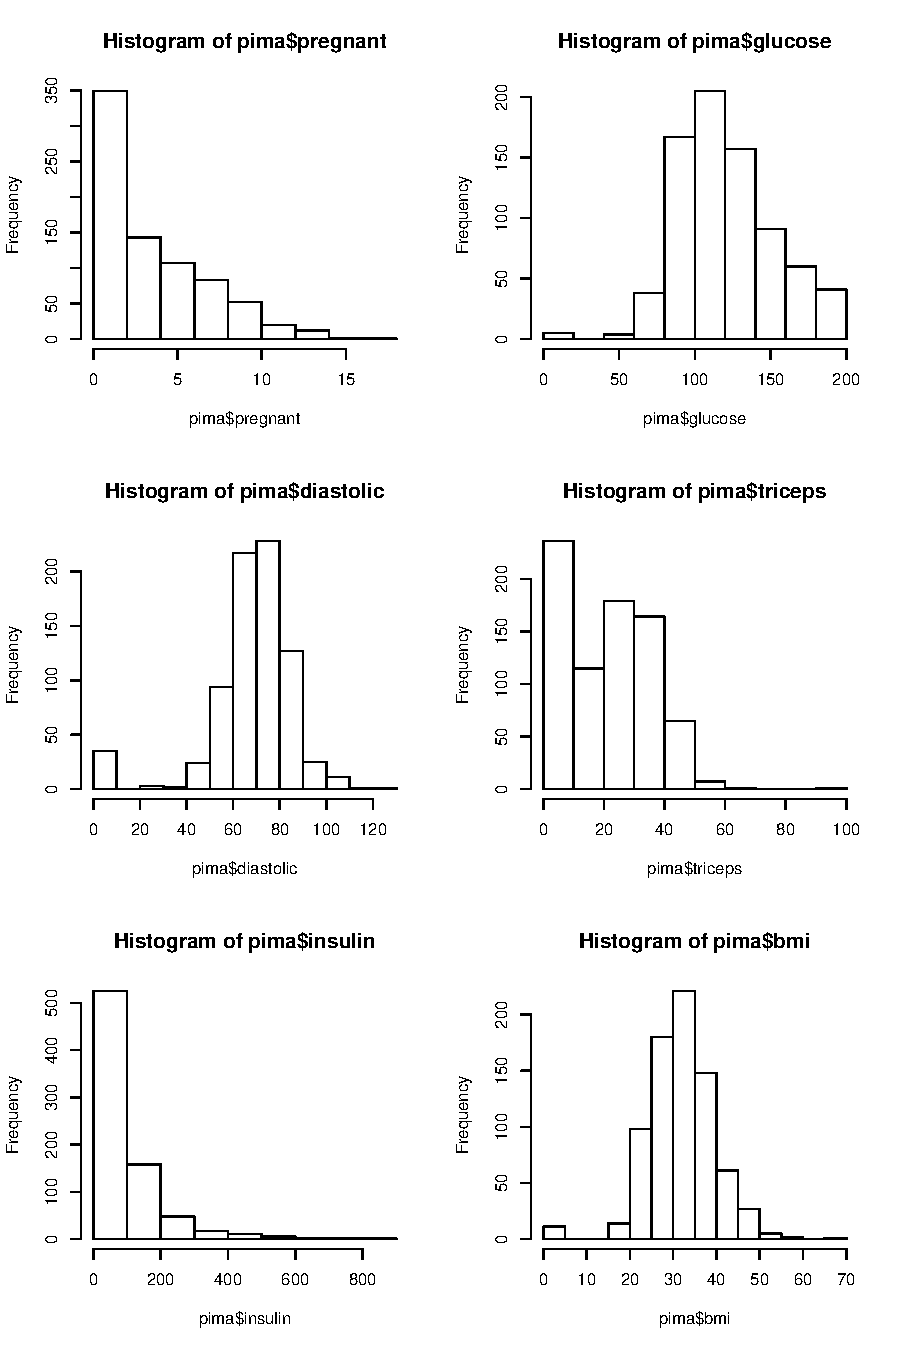
\includegraphics[width=1\linewidth]{figure/p3_a2-1} 

}



\end{knitrout}

As the result, histogram for \m{glucose}, \m{diastolic} and \m{bmi} all suggests that there are some weird 0 cases, which strongly suggests that they are missing values, and we should remove them.

\begin{knitrout}
\definecolor{shadecolor}{rgb}{1, 1, 1}\color{fgcolor}\begin{kframe}
\begin{alltt}
\hlcom{## remove weird 0's}
\hlstd{data} \hlkwb{<-} \hlstd{pima}
\hlstd{data} \hlkwb{<-} \hlstd{data[data}\hlopt{$}\hlstd{glucose} \hlopt{!=} \hlnum{0}\hlstd{, ]}
\hlstd{data} \hlkwb{<-} \hlstd{data[data}\hlopt{$}\hlstd{diastolic} \hlopt{!=} \hlnum{0}\hlstd{, ]}
\hlstd{data} \hlkwb{<-} \hlstd{data[data}\hlopt{$}\hlstd{bmi} \hlopt{!=} \hlnum{0}\hlstd{, ]}
\end{alltt}
\end{kframe}
\end{knitrout}

\subproblem{3.b}
Fit a model with the result of the diabetes test as the response and all the other variables as predictors. Can you tell whether this model fits the data?

\solution
\begin{knitrout}
\definecolor{shadecolor}{rgb}{1, 1, 1}\color{fgcolor}\begin{kframe}
\begin{alltt}
\hlstd{m1} \hlkwb{<-} \hlkwd{glm}\hlstd{(test} \hlopt{~} \hlstd{.,} \hlkwc{data} \hlstd{= data,} \hlkwc{family} \hlstd{= binomial)}
\hlkwd{summary}\hlstd{(m1)}
\end{alltt}
\begin{verbatim}
## 
## Call:
## glm(formula = test ~ ., family = binomial, data = data)
## 
## Deviance Residuals: 
##     Min       1Q   Median       3Q      Max  
## -2.6374  -0.7152  -0.4079   0.7214   2.4149  
## 
## Coefficients:
##               Estimate Std. Error z value Pr(>|z|)    
## (Intercept) -9.0572456  0.8276228 -10.944  < 2e-16 ***
## pregnant     0.1161430  0.0335394   3.463 0.000534 ***
## glucose      0.0369312  0.0039120   9.441  < 2e-16 ***
## diastolic   -0.0105289  0.0087177  -1.208 0.227137    
## triceps      0.0001526  0.0071103   0.021 0.982879    
## insulin     -0.0011241  0.0009266  -1.213 0.225066    
## bmi          0.0943048  0.0169173   5.574 2.48e-08 ***
## diabetes     1.0076042  0.3109647   3.240 0.001194 ** 
## age          0.0159706  0.0098765   1.617 0.105871    
## ---
## Signif. codes:  0 '***' 0.001 '**' 0.01 '*' 0.05 '.' 0.1 ' ' 1
## 
## (Dispersion parameter for binomial family taken to be 1)
## 
##     Null deviance: 931.94  on 723  degrees of freedom
## Residual deviance: 671.13  on 715  degrees of freedom
## AIC: 689.13
## 
## Number of Fisher Scoring iterations: 5
\end{verbatim}
\end{kframe}
\end{knitrout}

Here we fit the full model \m{m1} with residual deviance 671.1337505 on 715 degrees of freedom

It's hard to tell whether this model fits the data or not because in this problem $n_{i} = 1,~ \forall i$, so that the deviance doesn't converge to any distribution, hence we don't have an available statistical test for it. However, compared with the degrees of freedom, the residual deviance is relatively lower, which might suggests that this model is not bad.

\subproblem{3.c}
What is the difference in the odds of testing positive for diabetes for a woman with a BMI at the first quartile compared with a woman at the third quartile, assuming that all other factors are held constant? Give a confidence interval for this difference.

\solution
Note that the estimated coefficient for \m{bmi} is 0.094, suggesting that a unit increase in \m{bmi} with all other predictors held fixed increases the \textbf{log-odd} of testing positive for diabetes by 0.094 in average. 

Since the difference between the third quartile and the first quartile of \m{bmi} is $9.1$, the \textbf{log-odd} of testing positive for diabetes for a woman with a BMI at the third quartile will be larger than a woman at first quartile by $9.1 * 0.094 = 0.858$ in average, with all other predictors held fixed. Since the standard deviation of \m{bmi} is 0.0169, then a reasonable 95\% confidence interval for the difference in \textbf{log-odd} should be $(0.556, ~1.160)$

\subproblem{3.d}
Do women who test positive have higher diastolic blood pressures? Is the diastolic blood pressure significant in the regression model? Explain the distinction between the two questions and discuss why the answers are only apparently contradictory.

\solution
\begin{knitrout}
\definecolor{shadecolor}{rgb}{1, 1, 1}\color{fgcolor}\begin{kframe}
\begin{alltt}
\hlstd{diastolic_pos} \hlkwb{<-} \hlstd{data}\hlopt{$}\hlstd{diastolic[data}\hlopt{$}\hlstd{test} \hlopt{==} \hlnum{1}\hlstd{]}
\hlstd{diastolic_neg} \hlkwb{<-} \hlstd{data}\hlopt{$}\hlstd{diastolic[data}\hlopt{$}\hlstd{test} \hlopt{==} \hlnum{0}\hlstd{]}
\hlkwd{boxplot}\hlstd{(diastolic_pos, diastolic_neg,}
        \hlkwc{names} \hlstd{=} \hlkwd{c}\hlstd{(}\hlstr{"Positive"}\hlstd{,} \hlstr{"Negative"}\hlstd{),}
        \hlkwc{main} \hlstd{=} \hlstr{"Boxplot of Diastolic"}\hlstd{)}

\hlkwd{t.test}\hlstd{(diastolic_pos, diastolic_neg,} \hlkwc{alternative} \hlstd{=} \hlstr{"greater"}\hlstd{)}
\end{alltt}
\begin{verbatim}
## 
## 	Welch Two Sample t-test
## 
## data:  diastolic_pos and diastolic_neg
## t = 4.5294, df = 499.558, p-value = 3.704e-06
## alternative hypothesis: true difference in means is greater than 0
## 95 percent confidence interval:
##  2.762025      Inf
## sample estimates:
## mean of x mean of y 
##  75.24900  70.90737
\end{verbatim}
\end{kframe}

{\centering 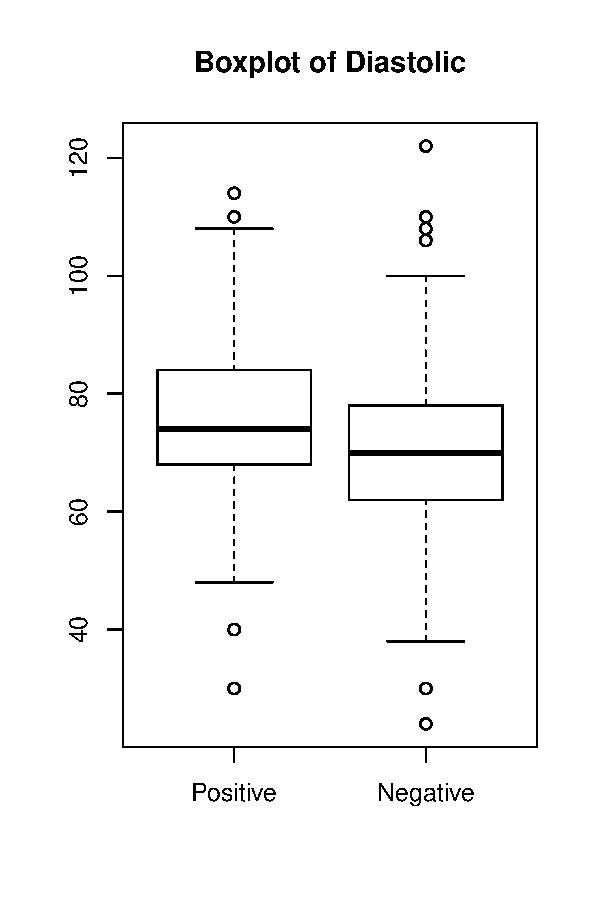
\includegraphics[width=.5\linewidth]{figure/p3_d-1} 

}



\end{knitrout}

First we draw a box-plot of \m{diastolic} blood pressures for women with different \m{test} result. Here we see that the the average diastolic level of women who tested positive only slightly higher than those who tested negative. Then we run t-test to determine whether the mean of \m{diastolic} from women who test positive is significantly greater than those who test negative. The resulting p-value suggests that women who test positive do have higher diastolic blood pressures. 

Then as what we see in the regression model, \m{diastolic} is not significant under $\alpha = 0.05$ level t-test.

Here is the distinction between the two questions:
\begin{itemize}
    \item the first question only consider the effect of \m{diastolic} over \m{test} result, where the effect of other predictors are ignored.
    \item the second question consider the effect of \m{diastolic} over the part of \m{test} that is not explained by other predictors.
\end{itemize}

In brief, the significance level of \m{diastolic} in the regression model is adjusted by other predictors, but when we talked about the first question, the effect of other predictors is ignored. So that the answers are only apparently contradictory.

\subproblem{3.e}
Perform diagnostics on the regression model, reporting any potential violations and any suggested improvements to the model.

\solution
First Let's check whether there are outliers included in the training dataset by using half-normal plot as follows:
\begin{knitrout}
\definecolor{shadecolor}{rgb}{1, 1, 1}\color{fgcolor}\begin{kframe}
\begin{alltt}
\hlkwd{halfnorm}\hlstd{(}\hlkwd{residuals}\hlstd{(m1),} \hlkwc{main} \hlstd{=} \hlstr{"Half-normal plot for m1"}\hlstd{)}
\end{alltt}
\end{kframe}

{\centering 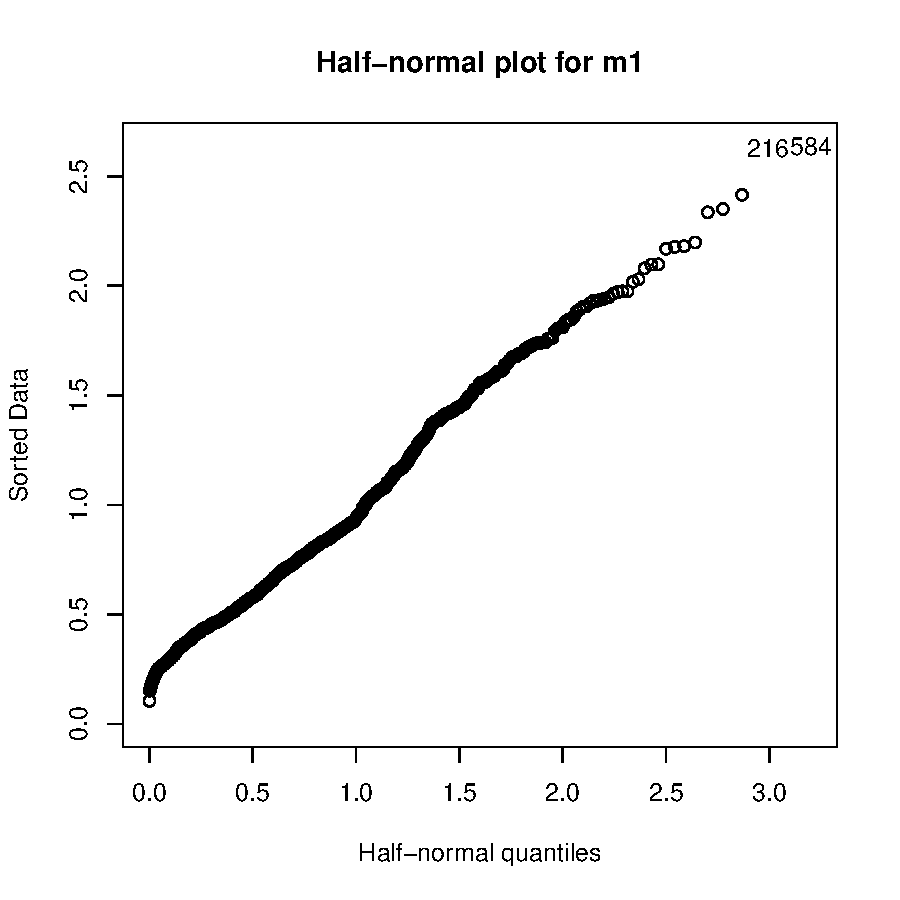
\includegraphics[width=.7\linewidth]{figure/p3_ep-1} 

}



\end{knitrout}

The half-normal plot suggests that the case 216 and 584 are outliers, hence we will remove them from the dataset.

More than that, here we can see that there are some predictors that are not significant enough in the regression model, so that we can apply AIC based stepwise regression on the full model to obtain a best reduced model.

\begin{knitrout}
\definecolor{shadecolor}{rgb}{1, 1, 1}\color{fgcolor}\begin{kframe}
\begin{alltt}
\hlstd{data} \hlkwb{<-} \hlstd{data[}\hlopt{-}\hlkwd{c}\hlstd{(}\hlnum{216}\hlstd{,}\hlnum{584}\hlstd{), ]} \hlcom{##Remove Outliers}
\hlstd{m1} \hlkwb{<-} \hlkwd{glm}\hlstd{(test} \hlopt{~} \hlstd{.,} \hlkwc{data} \hlstd{= data,} \hlkwc{family} \hlstd{= binomial)}
\hlstd{m0} \hlkwb{<-} \hlkwd{glm}\hlstd{(test} \hlopt{~} \hlnum{1}\hlstd{,} \hlkwc{data} \hlstd{= data,} \hlkwc{family} \hlstd{= binomial)}
\hlstd{m_AIC} \hlkwb{<-} \hlkwd{step}\hlstd{(m1,} \hlkwc{scope} \hlstd{=} \hlkwd{list}\hlstd{(}\hlkwc{lower} \hlstd{= m0,} \hlkwc{upper} \hlstd{= m1),}
              \hlkwc{trace} \hlstd{=} \hlnum{FALSE}\hlstd{,} \hlkwc{direction} \hlstd{=} \hlstr{"both"}\hlstd{)}
\hlkwd{summary}\hlstd{(m_AIC)}
\end{alltt}
\begin{verbatim}
## 
## Call:
## glm(formula = test ~ pregnant + glucose + bmi + diabetes + age, 
##     family = binomial, data = data)
## 
## Deviance Residuals: 
##     Min       1Q   Median       3Q      Max  
## -2.4771  -0.7018  -0.3901   0.6795   2.5106  
## 
## Coefficients:
##             Estimate Std. Error z value Pr(>|z|)    
## (Intercept) -9.73096    0.78020 -12.472  < 2e-16 ***
## pregnant     0.12044    0.03384   3.559 0.000372 ***
## glucose      0.03656    0.00367   9.963  < 2e-16 ***
## bmi          0.08821    0.01527   5.776 7.63e-09 ***
## diabetes     1.24331    0.31465   3.951 7.77e-05 ***
## age          0.01413    0.00963   1.467 0.142418    
## ---
## Signif. codes:  0 '***' 0.001 '**' 0.01 '*' 0.05 '.' 0.1 ' ' 1
## 
## (Dispersion parameter for binomial family taken to be 1)
## 
##     Null deviance: 930.25  on 721  degrees of freedom
## Residual deviance: 658.41  on 716  degrees of freedom
## AIC: 670.41
## 
## Number of Fisher Scoring iterations: 5
\end{verbatim}
\end{kframe}
\end{knitrout}

Note that there are only 5 predictors included in the AIC based reduced model, suggesting that not all variables are necessary in explaining the test result. The reduced model can be interpreted more easily and may achieve better generalization capability.

\subproblem{3.f}
Predict the outcome for a woman with predictor values 1, 99, 64, 22, 76, 27, 0.25, 25 (same order as in the dataset). Give a confidence interval for your prediction.

\solution
\begin{knitrout}
\definecolor{shadecolor}{rgb}{1, 1, 1}\color{fgcolor}\begin{kframe}
\begin{alltt}
\hlstd{newx} \hlkwb{<-} \hlstd{data[}\hlnum{1}\hlstd{,} \hlopt{-}\hlkwd{ncol}\hlstd{(data)]}
\hlstd{newx[}\hlnum{1}\hlstd{, ]} \hlkwb{<-} \hlkwd{c}\hlstd{(}\hlnum{1}\hlstd{,} \hlnum{99}\hlstd{,} \hlnum{64}\hlstd{,} \hlnum{22}\hlstd{,} \hlnum{76}\hlstd{,} \hlnum{27}\hlstd{,} \hlnum{0.25}\hlstd{,} \hlnum{25}\hlstd{)}
\hlstd{foo} \hlkwb{<-} \hlkwd{predict}\hlstd{(m_AIC,} \hlkwc{newdata} \hlstd{= newx,} \hlkwc{se.fit} \hlstd{=} \hlnum{TRUE}\hlstd{)}
\hlstd{ConfInterval} \hlkwb{<-} \hlkwd{ilogit}\hlstd{(}\hlkwd{c}\hlstd{(foo}\hlopt{$}\hlstd{fit} \hlopt{-} \hlnum{1.96} \hlopt{*} \hlstd{foo}\hlopt{$}\hlstd{se.fit,}
                         \hlstd{foo}\hlopt{$}\hlstd{fit} \hlopt{+} \hlnum{1.96} \hlopt{*} \hlstd{foo}\hlopt{$}\hlstd{se.fit))}
\hlstd{ConfInterval}
\end{alltt}
\begin{verbatim}
##         1         1 
## 0.0327988 0.0753943
\end{verbatim}
\end{kframe}
\end{knitrout}

Here we see the confidence interval for the prediction of the probability that the new women will be tested as positive is $(0.0327988, 0.0753943)$, and it should be predicted as negative.


\end{document}
